Rozpatrywać będziemy przestrzeń probabilistyczną $(\Omega,\mathcal{F},\Pra)$, czyli niech $\Omega$ to pewien niepusty zbiór, $\mathcal{F}$ to $\sigma$-ciało zdarzeń losowych, a $\Pra$ to funkcja $\Pra\colon\Omega\rightarrow[0,1]$. 

\begin{df}[\textit{n}-wymiarowa zmienna losowa]
	\label{df:n_wym_zmienna_losowa}
	\textit{n}-wymiarową zmienną losową nazywamy funkcję określoną na przestrzeni zdarzeń elementarnych $\Omega$ i przyjmującą wartości rzeczywiste:
	
	$$ X\colon \Omega \mapsto \mathbb{R}^{n}, $$

	taką, że
	
	$$ \{ \omega \colon X(\omega) < x) \} \in \mathcal{F},$$
	
	dla każdego $x \in \R.$
\end{df}

W całej pracy zakładać będziemy że poruszamy się w przestrzeni zmiennych ciągłych, ponieważ dotykać będziemy problematyki danych rynkowych o takim charakterze. Teoria kopuł jest rozwinięta co prawda również dla zmiennych dyskretnych (\cite{Genest_Discrete_Copulas}) i dorobiła się już ciekawych aplikacyjnych prac (np. \cite{Koopman_DiscreteCopula_HTF}, czy \cite{Shefzik_Weather}), jednak literatura jest tu zdecydowanie uboższa. Do opisu interesujących nas rozkładów dostępne będziemy więc mieć analityczne postaci ich dystrybuanty lub gęstości. Ponieważ często podaje się różne ich parametryzacje, w tabeli \ref{tab:przykladowe_zmienne_losowe} podajemy gęstości zmiennych losowych przewijających się w tej pracy. Ich wykresy widoczne są na wykresie \ref{fig:przykladowe_zmienne_losowe}.

Warto wspomnieć, że istnieją również użyteczne rozkłady, które nie dają się wyrazić za pomocą gęstości czy dystrybuanty. Najpopularniejszym przykładem mogą być rozkłady stabilne, gdzie jedyne czym może my się posługiwać to funkcja charakterystyczna.  \cite{Stable_Distributions1}, czy \cite{Stable_Distributions2} podają bardzo dobry przegląd teorii rozkładów stabilnych i pokazują ich przewagę w kontekście modelowania nie-gaussowskich zwrotów na rynkach finansowych.

\begin{table}[h]
	\caption{\textbf{Popularne jednowymiarowe zmienne losowe.} Tabela przedstawia dystrybuanty, oraz gęstości popularnych jednowymiarowych zmiennych losowych pojawiających się w tej pracy.}
	\label{tab:przykladowe_zmienne_losowe}
	\centering
	\begin{tabular}{ll|c|c}
		\hline
		\textbf{Rozkład} & \textbf{Oznaczenie} & \textbf{Nośnik} & \textbf{Gęstość} \\
		\hline
		Normalny & $\mathcal{N}(\mu, \sigma)$ & $\mathbb{R}$ & $\frac{1}{\sigma \sqrt{2 \pi}} \exp\big(-\frac{(x-\mu)^2}{2\sigma^2}\big)$\\ 
		T-studenta & $\text{t}(\mu, \sigma, \nu)$ & $\mathbb{R}$ & $ \frac{\Gamma(\frac{\nu + 1}{2})}{\Gamma(\frac{\nu}{2})\sqrt{\pi\nu}\sigma} \bigg[1 + \big(\frac{x - \mu}{\sigma}\big)^2\frac{1}{\nu}\bigg]^{-\frac{\nu + 1}{2}} $ \\ 
		Beta & $\text{Beta}(\alpha, \beta)$ & $[0, 1]$ & $ x^{\alpha - 1}(1 - x)^{\beta - 1}\frac{\Gamma(\alpha + \beta)}{\Gamma(\alpha)\Gamma(\beta)}$ \\ 
		Wykładniczy & $\text{Exp}(\lambda)$ & $\mathbb{R}^{+}$ & $ \lambda e^{-\lambda x}$ \\
		Gamma & $\mathcal{G}(\alpha, \beta)$ & $\mathbb{R}^+$ & $x^{\alpha - 1}e^{-\beta x}\frac{\beta^\alpha}{\Gamma(\alpha)}$\\ 
		
		\hline
	\end{tabular}
\end{table}

\begin{figure}[H]
	\centering
	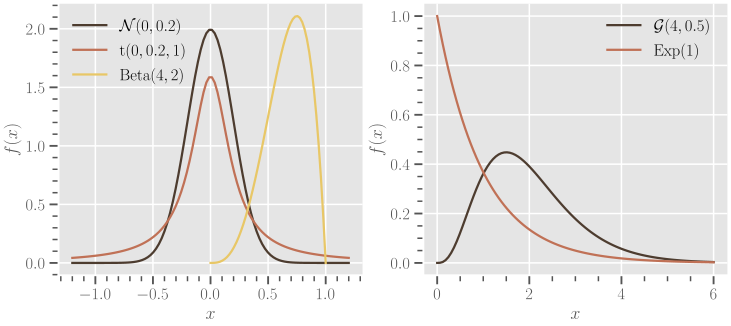
\includegraphics[width=\linewidth]{01_Rozklady_1D}
	\caption{Przykładowe gęstości zmiennych losowych z tabeli \ref{tab:przykladowe_zmienne_losowe}.\label{fig:przykladowe_zmienne_losowe}}
\end{figure}

Do opisu zmiennych losowych \emph{wielo}wymiarowych, oprócz gęstości łącznej rozkładu wyróżniamy dodatkowo gęstości warunkowe i brzegowe. Opisują one jak zachowuje się współrzędna wektora losowego, jeśli pozostałe z nich przyjmą pewne wartości, lub jeśli kompletnie wyłączymy ich wpływ.

\begin{df}[Rozkłady brzegowy]
	Rozpatrzmy d-wymiarową zmienną losową $\mathbf{X} = [X_1, X_2, \dots, X_d]$ o gęstości $f(x_1, \dots, x_d)$. Gęstość rozkładu brzegowego $X_j$ definiujemy jako:
	$$f_j(x_j)=\int_{-\infty}^{\infty}\dots\int_{-\infty}^{\infty} f(x_1, \dots, x_{j-1}, x, x_{j+1}, \dots, x_d)  dx_1\dots dx_{j-1} dx_{j+1} \dots dx_d.$$
\end{df}

\begin{df}[Rozkład warunkowy]
	Rozpatrzmy d-wymiarową zmienną losową $\mathbf{X} = [X_1, X_2, \dots, X_d]$ o gęstości $f(x_1, \dots, x_d)$. Gęstość rozkładu warunkowego $X_j \vert X_k$ definiujemy jako:
	$$f_{j|k}(x_j|x_k) = \frac{f(x_1, \dots, x_d)}{f_k(x_k)}.$$
\end{df}
